\documentclass[tikz,border=3pt]{standalone}
\usepackage{amsmath,lmodern}
\usetikzlibrary{arrows.meta,positioning,calc}
\definecolor{Ink}{HTML}{163047}
\definecolor{Teal}{HTML}{087F8C}
\definecolor{Clay}{HTML}{AD4C2B}
\begin{document}
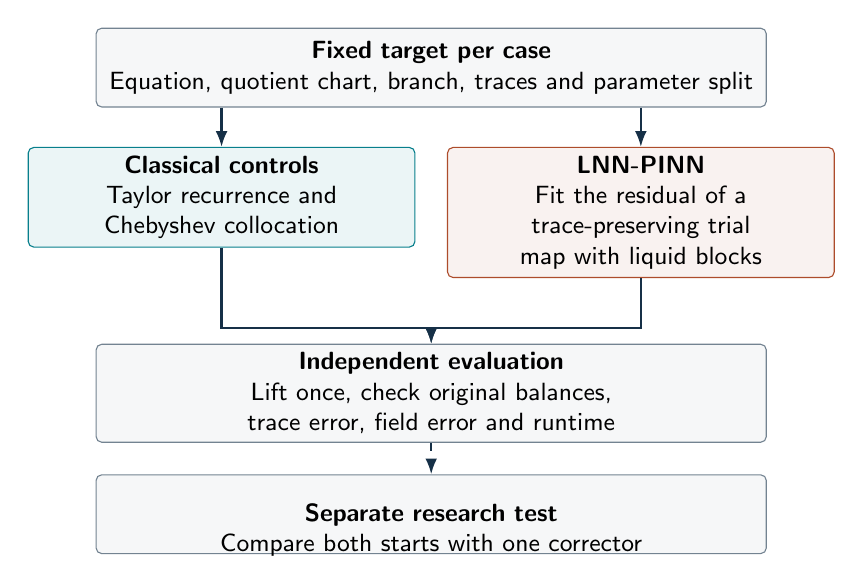
\begin{tikzpicture}[font=\sffamily\small,box/.style={draw=Ink!60,fill=Ink!4,rounded corners=2pt,align=center,text width=47mm,minimum height=10mm,inner sep=3pt},classical/.style={box,draw=Teal,fill=Teal!8},learn/.style={box,draw=Clay,fill=Clay!7},edge/.style={-{Latex[length=2mm]},draw=Ink,thick}]
\node[box,text width=83mm] (freeze) {\textbf{Fixed target per case}\\Equation, quotient chart, branch, traces and parameter split};
\node[classical,below left=5mm and 2mm of freeze.south] (base) {\textbf{Classical controls}\\Taylor recurrence and Chebyshev collocation};
\node[learn,below right=5mm and 2mm of freeze.south] (nn) {\textbf{LNN-PINN}\\Fit the residual of a trace-preserving trial map with liquid blocks};
\node[box,text width=83mm,below=30mm of freeze.south] (check) {\textbf{Independent evaluation}\\Lift once, check original balances, trace error, field error and runtime};
\node[box,text width=83mm,below=4mm of check,text depth=0.3ex] (future) {\textbf{Separate research test} \\Compare both starts with one corrector};
\draw[edge] (freeze.south -| base.north) -- (base.north);
\draw[edge] (freeze.south -| nn.north) -- (nn.north);
\draw[edge] (base.south) |- ([yshift=2mm]check.north) -- (check.north);
\draw[edge] (nn.south) |- ([yshift=2mm]check.north) -- (check.north);
\draw[edge,dashed] (check)--(future);
\end{tikzpicture}
\end{document}
